\documentclass{exam}
\usepackage{mainExam}

\title{Contrôle}
\date{14 Mars 2025}
\author{Seconde 9}

\begin{document}
\maketitle
\instructions{autorisée}
\begin{questions}
\vspace*{0.5cm}
\titledquestion{Fonctions}[5]
On s'intéresse aux bénéfices d'une entreprise de fabrication de cosmétiques. On note $C(x)$ la chiffre d'affaire \textit{(en centaine d'euros)} de l'entreprise après avoir produit $x$ litres de vernis.
\begin{parts}
\part On suppose que $C(x) = 8x - 5$
\begin{subparts}
\subpart[1] Calculer l'image de $2$ et de $0,5$.
\subpart[1] Pour quelle quantité de vernis l'entreprise gagne-t-elle \num{300} € ? Et \num{650} € ?
\end{subparts}
\part On suppose maintenant que la courbe représentative $\mathcal{C}_C$ de la fonction $C$ est donnée ci-dessous :
\begin{center}
\includegraphics[width=0.9\textwidth]{fonction.png}
\end{center}
\begin{subparts}
\subpart[0,5] Donner les bénéfices de l'entreprise, en centaine d'euros, quand elle produit $3$ litres de vernis.
\subpart[0,5] Même question pour $17$ litres de vernis.
\subpart[1] L'entreprise a gagné \num{400} €. Combien de litres de vernis a-t-elle produite ?
\subpart[1] Même question pour \num{250} €.
\end{subparts}
\end{parts}
\vspace*{0.5cm}
\titledquestion{Valeur absolue et distance}[5]
\begin{parts}
\part[1] Calculer les valeurs absolues suivantes :
\begin{subparts}
\subpart $\abs{2}$
\subpart $\abs{-3}$
\subpart $\abs{0}$
\subpart $\abs{-\pi}$
\end{subparts}
\part[1.5] Résoudre les équations suivantes :
\begin{subparts}    
\subpart $\abs{x} = 6$
\subpart $\abs{t} = -1$
\subpart $\abs{3y + 1} = 10$
\end{subparts}
\part[1] Rappeler la définition de la distance entre deux nombres $a$ et $b$.
\part[1.5] Résoudre les équations suivantes, en donnant l'ensemble des solutions sous la forme d'un intervalle. On pourra s'aider d'un dessin.
\begin{subparts}
\subpart $\abs{x - 3} \leq 3$
\subpart $\abs{x - 1,2} \leq 7$
\subpart $\abs{x + 2} \leq 0,2$
\end{subparts}
\end{parts}
\vspace{0.5cm}
\titledquestion{Intervalles}[5]
\begin{parts}
\part[3] Compléter le tableau suivant :
\vspace*{0.5cm}
\begin{center}
\begin{tabular}{|m{3cm}|m{3cm}|m{4cm}|}
\hline
Intervalle&Inégalité&Représentation graphique\\
\hline
$[12;15]$&&\begin{tikzpicture}\draw[->] (0,-0.5) -- (3.9,-0.5);
\draw node (0,0) {};\end{tikzpicture}\\[0.5cm]
\hline
&$x \leq 4$&\begin{tikzpicture}\draw[->] (0,-0.5) -- (3.9,-0.5);
\draw node (0,0) {};\end{tikzpicture}\\[0.5cm]
\hline
&&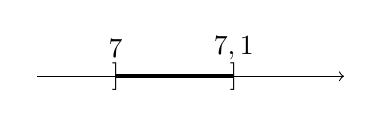
\begin{tikzpicture}\draw[->] (0,-0.5) -- (3.9,-0.5);
\draw node (0,0) {};
\draw (1,-0.15) node {$7$}; 
\draw (1,-0.5) node {$]$};
\draw (2.5,-0.15) node {$7,1$}; 
\draw (2.5,-0.5) node {$]$};
\draw[ultra thick] (1,-0.5) -- (2.5,-0.5); \end{tikzpicture}\\[0.5cm]
\hline
$]-6,25;+\infty[$&&\begin{tikzpicture}\draw[->] (0,-0.5) -- (3.9,-0.5);
\draw node (0,0) {};\end{tikzpicture}\\[0.5cm]
\hline
&$22 \leq x < 33$&\begin{tikzpicture}\draw[->] (0,-0.5) -- (3.9,-0.5);
\draw node (0,0) {};\end{tikzpicture}\\[0.5cm]
\hline
&&
\begin{tikzpicture}\draw[->] (0,-0.5) -- (3.9,-0.5);
\draw node (0,0) {};
\draw (2,-0.15) node {$\sqrt{2}$}; 
\draw (2,-0.5) node {$[$};
\draw[ultra thick] (2,-0.5) -- (3.9,-0.5); \end{tikzpicture}\\[0.5cm]
\hline
\end{tabular}
\end{center}
\part On dit qu'un intervalle $[a;b]$ est \textbf{inclus} dans un intervalle $[c;d]$ si et seulement si tout nombre $x$ appartenant à $[a;b]$ appartient aussi forcément à $[c;d]$.
\begin{subparts}
\subpart[0.5] L'intervalle $[1;5]$ est-il inclus dans l'intervalle $[0;6]$ ?
\subpart[1.5] Soient $a,b,c,d$ quatre nombres réels quelconques. Montrer que si $c \leq a$ et que si $b \leq d$, alors l'intervalle $[a;b]$ est inclus dans l'intervalle $[c;d]$. On pourra justifier à l'aide d'une représentation graphique.
\end{subparts}
\end{parts}
\vspace*{0.5cm}
\vspace*{0.5cm}
\titledquestion{Décimaux, rationnels et irrationnels}[5]
\begin{parts}
\part[1.5] Pour chacun des nombres suivants, dire s'il est décimal, rationnel et/ou réel.
\begin{subparts}
\subpart $\dfrac{4}{25}$
\subpart $-0,78787878\dots$
\subpart $\dfrac{1}{3}$
\subpart $\sqrt{2}$
\subpart $0,65$
\subpart $\pi$
\end{subparts}
\part On souhaite montrer qu'un nombre dont le développement décimal est périodique infini est rationnel. On teste avec l'exemple suivant $A = 0.656565656565\dots$.
\begin{subparts}
\subpart[0.5] Justifier que $100A = 65 + A$.
\subpart[1] Donner la solution de cette équation sous forme de fraction. En déduire que $A$ est rationnel.
\end{subparts}
\part[2] En suivant la même méthodologie que la question précédente, trouver à quelle fraction sont égaux les nombres $B = 0,9797979797\dots$ et $C=0,123123123\dots$.
\end{parts}

\end{questions}
\end{document}